%-*- mode: LaTeX; -*-

%Consists of Si and C atoms, crystal. (Arranged periodically)
%There exists many (Citation?) different kinds of polytypes
%Polytypes can be thought of as stacking sequence of hexagonal layers
%Base is one C and one Si
%Si and C faces, what is that? [Do I need this?]
%If I do anything on bulk, then I should discuss planes here. (Since the goal is to have (100) plane).

%The atoms are bonded together by covalent bonds.
%The band structure is shown...
%Indirect band gap of...

%Some relevant properties
%Mobility
%Dielectric constant

%Nitrogen as background doping
%Possible acceptors are
%Boron doping gives good band diagram as seen...


\chapter{An introduction to silicon carbide}
\label{sec:sic}
This chapter describes the relevant properties of SiC. Section \ref{sec:crystal_structure} describes the atomic arrangement in the material, and some different arrangements are discussed. Section \ref{sec:band_structure} discusses the energy band structure of 3C-SiC. Finally section \ref{sec:doping_in_3C} describes the mechanism and some effects of doping in 3C-SiC. 

\section{Crystal structure}
\label{sec:crystal_structure}
Silicon carbide is a crystalline material consisting of silicon and carbon atoms. The crystalline nature of the material means that the atoms are arranged in a periodically repeating structure called a \emph{lattice}. For given chemical elements there may be several different ways to arrange the atoms in a lattice, i.e. different chemical compounds of the same types of atoms. This is called \emph{polytypism}, where the different lattice structures are called \emph{polytypes} of the material. SiC has a large number of different polytypes. There are more than 250 known polytypes of SiC \cite{Cheung2006}. The different polytypes can be described as different stacking orders of layers of atoms \cite{Mirgorodsky1995}. Figure \ref{fig:hex} shows one such layer. Here each circle symbolizes one carbon and one silicon atom, displaced a small distance from each other. This pair of atoms is called the \emph{base} of the crystal. 

\begin{figure}[h]
\begin{center}
\includegraphics[scale=1]{lattice2.pdf}
\caption{Atomic arrangement of the atoms in each layer. Here each sphere corresponds to one carbon and one silicon atom, as shown by the arrow. 
\label{fig:hex}}
\end{center}
\end{figure}

The marked hexagon in figure \ref{fig:hex} marks an area of the crystal which can be used to define the different polytypes. Figure \ref{fig:stacking1} shows the same area but with different placements of the base atoms. Again each sphere is one crystal base. The three different placements A, B and C describe how each layer is placed compared to the one above. It should be noted that the plane in figure \ref{fig:hex} is the same as A in figure \ref{fig:stacking1}.

\begin{figure}[h]
\begin{center}
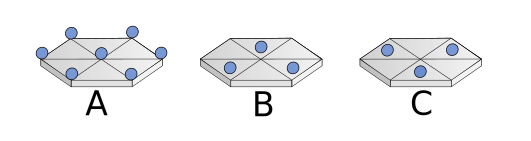
\includegraphics[scale=0.7]{hex5.pdf}
\caption{Different atomic placements for the layers
\label{fig:stacking1}}
\end{center}
\end{figure}

The stacking orders of three of the most common polytypes is shown in figure \ref{fig:poly}. The depicted orders of the layers refers to one period in the periodic structure. The names for the different polytypes are stated at the top of the figure. The digit in the name refers to the number of layers of a period and the letter denotes the crystal symmetry. The letter \emph{H} denotes the hexagonal polytypes, whereas \emph{C} stands for the cubic polytype. Another common polytype is the 6H-SiC, which thus is a hexagonal structure with a period of six base layers. It should be noted that the 2H structure is the wurtzite structure and the 3C is the zincblende structure.  

\begin{figure}[h]
\begin{center}
\includegraphics[scale=0.8]{poly.pdf}
\caption{Stacking order for the three most simple polytypes. 
\label{fig:poly}}
\end{center}
\end{figure}

\section{Band structure}
\label{sec:band_structure}

\begin{figure}[h]
\begin{center}
\includegraphics[scale=1]{band_diagram.pdf}
\caption{The band diagram of SiC at ambient conditions for different positions in the Brillouin zone. The indirect and direct band gaps are marked in the figure. The marked area is the band gap. The energy levels have been obtained using the pseudopotential method, as described in \cite{Aourag1994}.
\label{fig:band}}
\end{center}
\end{figure}

%\section{Some properties}
%\label{sec:}




\section{Doping in 3C}
\label{sec:doping_in_3C}

























